\section{Descripción modular del código} % Seções são adicionadas para organizar sua apresentação em blocos discretos, todas as seções e subseções são automaticamente exibidas no índice como uma visão geral da apresentação, mas NÃO são exibidas como slides separados.


\begin{frame}{Módulos}
    División del proyecto:
    \begin{itemize}
        \item \textbf{Catjack.rkt}: flujo principal y menús de juego.
        \item \textbf{gráficos.rkt}: implementación de los elementos gráficos usando \textit{graphics}.
        \item \textbf{letras.rkt}: implementación de tipografía.
        \item \textbf{figuras.rkt}: mapas de puntos para los gráficos.
        \item \textbf{juego.rkt}: implementación de turnos y lógica de juego.
    \end{itemize}
\end{frame}

%------------------------------------------------
\subsection{Gráficos}
\begin{frame}{Gráficos}
	\begin{itemize}
		\item \textbf{Principio básico}: mapas de puntos escalables y desplazables.
		\[
		(x', y') = \left( (x - r_x) \cdot s_x + c_x, (y - r_y) \cdot s_y + c_y \right)
		\]
	\end{itemize}
	\begin{center}
		\small
		\item $r_i \equiv$ centroide del eje $i$
		\item $s_i \equiv$ escala del eje $i$
		\item $c_i \equiv$ centro hacia el que desplazar el punto en el eje $i$
	\end{center}
\end{frame}



%------------------------------------------------
\begin{frame}{Gráficos (2)}
    Figuras generadas mediante las siguientes funciones:
    \begin{itemize}
        \item Puntos de \textbf{tangencia} de una circunferencia por un punto.
        \item Puntos de los \textbf{cuadrantes} de una circunferencia (cuarta parte de la figura cortada por los ejes x e y): 
        \begin{itemize}
            \item \textbf{Posición}: arriba derecha, abajo izquierda, etc.
            \item \textbf{Sentido}: horario o antihorario.
        \end{itemize}
    \end{itemize}
\end{frame}

%------------------------------------------------
\begin{frame}{Gráficos (3)}
    Jerarquía de creación de figuras de simple a general:
    \begin{enumerate}
        \item \textbf{Elementos sencillos}
        \begin{itemize}
            \item \textbf{Palos} de las cartas (pica, diamante, trébol y corazón).
            \item \textbf{Valores} de las cartas (A, 1, 2, 3, ... Q, K).
            \item La \textbf{pata} del gato.
            \item \textbf{Tipografía}
            \item \textbf{Logotipo} de la carátula.
        \end{itemize}
        \item \textbf{Cartas}: 
        \begin{itemize}
            \item Carta \textbf{por delante}: palo y valor.
            \item Carta \textbf{por detrás}: con el logo. 
        \end{itemize}
        \item \textbf{Animaciones}: 
        \begin{itemize}
            \item Mover carta con pata.
            \item Mover pata.
        \end{itemize}
        
    \end{enumerate}
\end{frame}

%------------------------------------------------

\begin{frame}{Gráficos (3.1)}
    \textit{Problema} con las \textbf{animaciones}: siempre dibuja encima de lo previamente dibujado.
    \begin{itemize}
        \item \textbf{Solución}: limpiar el fondo antes de imprimir el siguiente frame de la animación.
        \item \textbf{Inconveniente}: solución factible solo para \textbf{fondos de un color}.
        \item \textbf{Posible mejora}: implementar sistema de \textbf{capas} de profundidad mediante listas (motor gráfico 2D).
    \end{itemize}
\end{frame}

%------------------------------------------------

\begin{frame}{Gráficos (4)}
    \begin{enumerate}[4]
        \item \textbf{Elementos de la mesa}
        \begin{itemize}
            \item \textbf{Botones}: plantarse, pedir, doblar.
            \item \textbf{Contadores}: fichas o rondas ganadas del jugador y del crupier.
            \item \textbf{Fondo} representando el tapete y mesa.
        \end{itemize}
        \item \textbf{Menús interactivos}:
        \begin{itemize}
            \item Menús de \textbf{inicio}: \textbf{carátula}, \textbf{modo} de juego, \textbf{rondas} a jugar.
            \item Seleccionar \textbf{fichas a apostar}.
            \item Indicar número de \textbf{fichas iniciales} (entrada por teclado). 
        \end{itemize}
    \end{enumerate}
\end{frame}

%------------------------------------------------

\begin{frame}{Gráficos (5)}
    \begin{figure}
        \centering
        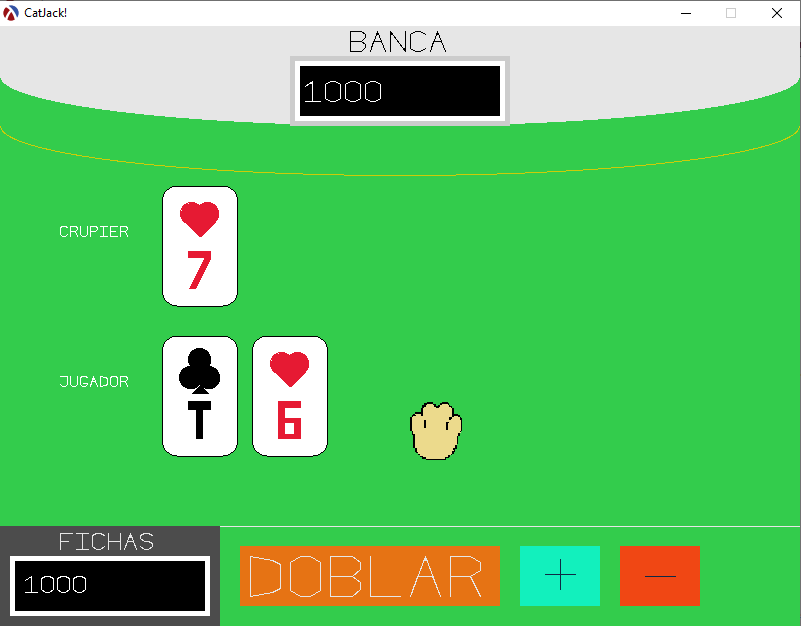
\includegraphics[width=0.5\linewidth]{img/mesa.png}
        \caption{Mesa de CatJack}
        \label{fig:enter-label}
    \end{figure}
\end{frame}

%------------------------------------------------
\subsection{Letras}
\begin{frame}{Letras}
La librería \textbf{\textit{graphics}} implementa impresión de cadenas, pero con poca \textbf{adaptabilidad}.
    \begin{itemize}
        \item \textbf{Solución}: implementar una tipografía completamente \textbf{manejable}.\\
    \end{itemize}
    
    Implementación compuesta por
    \begin{itemize}
        \item \textbf{Mapas de puntos} de cada símbolo disponible ([0-9A-ZÑ.+-]).
        \item Funciones de \textbf{impresión de cadena} que permita adaptar tamaño, color y posición.
    \end{itemize}
    
\end{frame}

%------------------------------------------------
\subsection{Juego}
\begin{frame}{Juego}
    El juego es \textbf{Point and click} (mecánica basada en ratón).\\
    El elemento básico del juego es el \textbf{botón}.\\
    \begin{itemize}
        \item Problema: \textbf{\textit{graphics}} no implementa botones.
        \item \textbf{Solución}: capturar clics y evaluar coordenadas de impacto.
        \begin{itemize}
            \item \textbf{Botones circulares}: región delimitada por distancia euclidiana.
            \item \textbf{Botones rectangulares}: región delimitada por coordenadas.
        \end{itemize}
    \end{itemize} 
\end{frame}

%------------------------------------------------
\begin{frame}{Juego (2)}
    Funcionalidades del juego:
    \begin{itemize}
        \item \textbf{Mazo}: se implementa un mazo de $52 \times 4$ cartas (usando listas) y la función de mezclar baraja.
        \item \textbf{Fichas iniciales}: se determinan las mismas para el \textbf{jugador} y para el \textbf{crupier}.    
        \item \textbf{TDAs}:
        \begin{itemize}
            \item \textbf{Jugada}: compuesto por la \textit{mano, fichas disponibles} y \textit{apuesta realizada}.
            \item \textbf{Ronda}: compuesto por \textit{ganador, mazo, fichas del jugador y fichas del crupier}.
        \end{itemize}
        \item \textbf{Reparto inicial}: se reparten dos cartas al jugador y una al crupier.
        \item \textbf{Determinar apuesta}: se determina la apuesta a realizar.
    \end{itemize}
\end{frame}
%------------------------------------------------
\begin{frame}{Juego (3)}
\begin{itemize}
    \item \textbf{Turno jugador}: opciones del jugador.
    \item \textbf{Turno del crupier}: saca cartas hasta tener una mano igual o mayor a 17.
    \item \textbf{Ronda}: se integra el reparto inicial, el turno del jugador, el turno del crupier y el resultado. Los \textbf{contadores} muestran fichas o rondas ganadas según el \textbf{modo de juego}. 
    \item \textbf{Blackjack}: se implementa el juego en dos funciones distintas:
    \begin{itemize}
        \item \textbf{blackjack-fichas}
        \item \textbf{blackjack-ganar}
    \end{itemize}
\end{itemize}
\end{frame}